\documentclass{article}
\usepackage{graphicx}
\begin{document}
\pagenumbering{gobble}
\begin{enviroment}
\end{enviroment}
\thispagestyle{empty}
\begin{center}
{\Large \bf Universidade Federal do Esp\'irito Santo\\[5pt]
Departamento de Inform\'atica
\end{center}
\vspace
*
{\stretch{1}}
\begin{center}
{\huge \bf 
2\b o Trabalho de Algoritmos Num\'ericos:\\
M\'etodos de Interpola\c c\~ao e de Integra\c c\~ao

\end{center}
\vspace
*
{\stretch{1}}
\begin{flushright}
Alunos: Matheus H. Risso e Pedro P. Ladeira\\
Professor: Prof. Dr. Thomas W. Rauber
\end{flushright}
\vspace
*
{\stretch{1}}
\begin{center}\begin{minipage}{12cm}
Trabalho da disciplina de Algoritmos Num\'ericos I, 
ministrada pelo Professor Dr. Thomas W. Rauber como forma de avalia\c c\~ao;
Universidade Federal do Esp\'irito Santo, 2016/1.
\end{minipage}\end{center}
\vspace
*
{\stretch{1}}
\centerline{\bf Vit\'oria-ES, 1 de Julho de 2016}
\vspace
*
{\stretch{1}}

\newpage
\pagenumbering{arabic}
\renewcommand{\contentsname}{Sum\'ario}
\tableofcontents

\newpage

\section{Introdu\c c\~ao}
\paragraph{} Denomina-se interpola\c c\~ao polinomial o processo de interpola\c c\~ao em que a fun\c c\~ao interpoladora \'e um polin\^omio.
Neste trabalho utilizaremos diversos n\'os (x,y) correspondentes a uma determinada fun\c c\~ao e encontraremos o polin\^omio p(x) correspondente
a fun\c c\~ao. Para tal utilizaremos as t\'ecnicas da matriz de Vandermonde e de Splines C\'ubicos.
\paragraph{} Este trabalho tamb\'em apresentar\'a t\'ecnicas de integra\c c\~ao aproximada. Ser\~ao apresentadas e comparadas a solu\c c\~ao 
anal\'itica a t\'ecnica dos trap\'ezios repetida e a t\'ecnica de 1/3 de simpson.
\newpage
\section{Objetivos}
\paragraph{}Este trabalho tem como objetivo entender e comparar diversos m\'etodos num\'ericos quanto a efici\^encia em se aproximar de solu\c c\~oes anal\'iticas e 
os aplicar num problema pr\'atico.
\paragraph{}Para isso utilizaremos a ferramenta computacional Octave GNU para criar fun\c c\~oes que descrevem os m\'etodos num\'ericos citados na especifica\c c\~ao.
Al\'em disso cuidaremos para que o c\'odigo seja compat\'ivel tanto com Octave como com o MATLAB.

\newpage
\section{Metodologia}
\paragraph{}Utilizando o material descrito na especifica\c c\~ao do trabalho entendemos cada m\'etodo e criamos fun\c c\~oes que descrevem cada um deles.
	\subsection{M\'etodos de Interpola\c c\~ao}
		\subsubsection{Vandermonde}
		C\'odigo fonte que descreve o m\'etodo de Vandermonde de interpola\c c\~ao polinomial, dados os n\'os em forma de string t corrensponde aos xs e 
		y aos ys
			\begin{figure}[h!]
			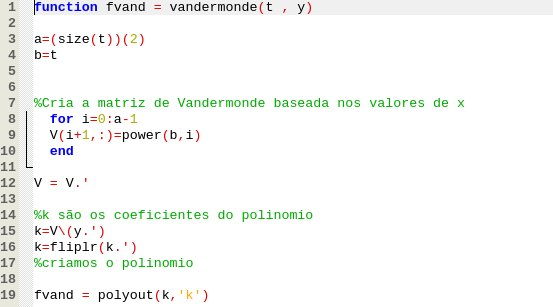
\includegraphics[width=\linewidth]{Vandermonde.jpg}
			\caption{Interpola\c c\~ao pela matriz de Vandermonde}
			\end{figure}
\newpage
		\subsubsection{Splines C\'ubicos}
		C\'odigo fonte que descreve o m\'etodo de interpolação polinomial por Splines C\'ubicos, dados os n\'os em forma de string t corrensponde aos xs e 
		y aos ys
			\begin{figure}[h!]
			\includegraphics[width=\linewidth]{Splines.jpg}
			\caption{M\'etodo de Interpola\c c\~ao polinomial por Splines C\'ubicos}
			\end{figure}
\newpage
\subsection{M\'etodos de Integra\c c\~ao}
		\subsubsection{M\'etodo dos Trap\'ezios repetidos}
		C\'odigo fonte que descreve o m\'etodo dos Trap\'ezios repetidos dada a fun\c c\~ao (funcao), os limites (a e b) e o n\'umero de 
		subdivis\~oes(n)
			\begin{figure}[h!]
			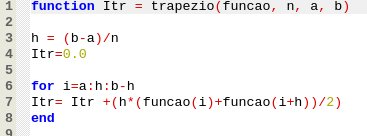
\includegraphics[width=\linewidth]{Trapezio.jpg}
			\caption{M\'etodo dos Trap\'ezios repetidos}
			\end{figure}
\newpage
		\subsubsection{M\'etodo 1/3 de Simpson}
		C\'odigo fonte que descreve o m\'etodo de Simpson de integração, dado a fun\c c\~ao(funcao), limites de integra\c c\~ao(a e b), 
		e o n\'umero de subdivis\~oes (n).
			\begin{figure}[h!]
			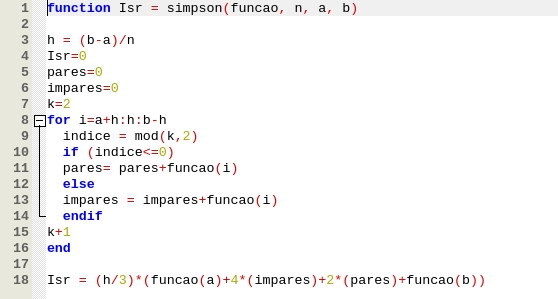
\includegraphics[width=\linewidth]{Simpson.jpg}
			\caption{M\'etodo 1/3 de Simpson}
			\end{figure}
\newpage
\section{Resultados e Avalia\c c\~oes}
	\subsection{Tabelas de Integra\c c\~ao}
	\paragraph{}Utilizando as t\'ecnicas de integra\c c\~ao dos trap\'ezios repetidos e de 1/3 de simpson pudemos observar que a t\'ecnica dos
	trap\'ezios \'e bem mais eficiente que a 1/3 de simpson. Abaixo as tabelas comparativas:
	\begin{figure}[h!]
		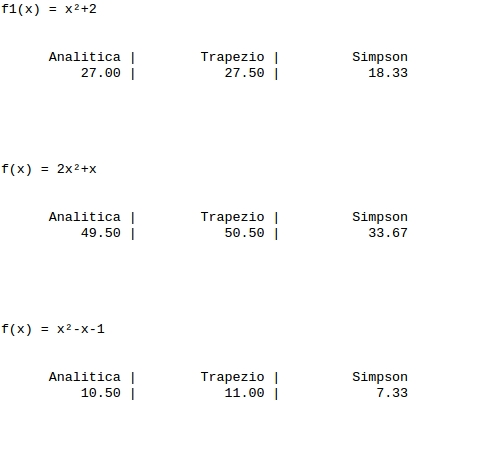
\includegraphics[width=\linewidth]{TabelaInts.jpg}
		\caption{Tabelas dos resultados obtidos a partir das t\'ecnicas}
		\end{figure}
\newpage
	\subsection{Gr\'aficos dos Polin\^omios}
	\begin{figure}[h!]
		\includegraphics[width=\linewidth]{Graficos.jpg}
		\caption{Gr\'afico sobreposto da fun\c c\~ao anal\'itica e dos metodos de interpola\c c\~ao}
		\end{figure}
\newpage
\section{Refer\^encias Bibliogr\'aficas}
\begin{itemize}
\item
https://pt.wikipedia.org/wiki/Interpola\%C3\%A7\%C3\%A3o\_polinomial
\item
https://pt.wikipedia.org/wiki/Integra\%C3\%A7\%C3\%A3o\_num\%C3\%A9rica
\end{itemize}
\newpage
\end{document}